\chapter{Objetivos}\label{cap.objetivos}
En este capitulo se presentaran los objetivos planteados para este proyecto, los requisitos marcados y la metodología utilizada para alcanzarlos.

\section{Objetivos}
La principal meta de este trabajo es la de enriquecer con tecnologías web las herramientas robóticas existentes en la plataforma JdeRobot. Para alcanzar este objetivo, se ha dividido el trabajo en tres partes: 
\begin{itemize}
\item Modificar los tres visores elaboradas mediante tecnologías web existentes en la plataforma JdeRobot, CameraViewjs, KobukiViewerjs y UavViewerjs, para su utilización con el middleware ROS, además de ICE como hasta ahora.
\item Elaborar un nuevo driver robótico utilizando tecnologías web, cuyo cometido sera el de servidor de imágenes a los distintos visores existentes en JdeRobot. 
\item Creación mediante tecnologías web, de un nuevo visor, que permitirá la visualización de elementos 3D (puntos, líneas y modelos 3D) que utilizara como middleware de comunicación, ICE.
\end{itemize}
Además, se ha utilizado el framework Electron en todos ellos para posibilitar que, además de usando un navegador, se puedan ejecutar como si de una aplicación de escritorio se tratase.

\section{Requisitos}
Los requisitos que se han tenido en cuenta a la hora de desarrollar todo el software de este trabajo han sido los siguientes:
\begin{itemize}
\item El sistema operativo utilizado ha sido Ubuntu 16.04 LTS y macOS HighSierra, además, gracias a utilizar tecnologías web, todos los componentes pueden ser ejecutados en cualquier sistema operativo.
\item Se ha utilizado la versión de NodeJS 8.9.1 y de NPM 6.4.0.
\item Los middleware utilizados han sido JdeRobot en su versión 5.6.4, ROS en su versión Kinetic y ICE en su versión 3.6.4.
\item Para permitir ejecutar la ejecución de todo los elementos como una aplicación de escritorio, se ha utilizado Electron en la versión 1.8.
\item Se ha utilizado HTML5, CSS3 y JavaScript para la elaboración de los software.
\item El funcionamiento con el middleware ROS sera mediante la biblioteca Rosbridge Server de RobotWebTools.
\end{itemize}

\section{Metodología}
La metodología elegida para la ejecución del trabajo ha sido el desarrollo en espiral. Se trata de uno de los modelos más utilizados en el desarrollo de software, y consiste en la realización de una serie de cilcos o iteraciones que se repiten en forma de espiral.
\begin{figure}[H]
  \begin{center}
    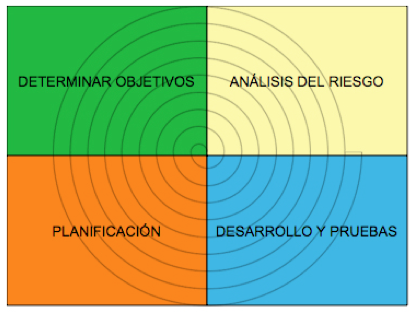
\includegraphics[width=0.8\textwidth]{figures/desarrolloespiral.png}
		\caption{Modelo de desarrollo en espiral}
		\label{fig.desarrolloespiral}
		\end{center}
\end{figure}
Cada iteración o ciclo esta formado por cuatro etapas.
\begin{enumerate}
\item Determinación de los objetivos a alcanzar para que el ciclo sea finalizado de manera exitosa.
\item Analizar los riegos que conlleva las elecciones tomadas para realizar el desarrollo, y establecer alternativas para solventar los posibles inconvenientes.
\item Desarrollar y probar los objetivos establecidos en la primera fase.
\item Planificar las siguientes etapas del proyecto, teniendo en cuenta los resultados obtenidos en esta interacción.
\end{enumerate}
De cara a poder llevar un mejor control del trabajo, se han tenido reuniones semanales con el tutor, en las que se marcaban los objetivos para la siguiente semana, se exponían dudas o posibles problemas  así como se establecen posibles alternativas, y se revisaba el trabajo previo. Con estas reuniones semanales se consigue tener flujo de trabajo constante y fluido, disminuyendo la posibilidad de quedar bloqueado en algún punto durante un largo periodo de tiempo.

Además, se ha elaborado un bitácora en la mediawiki\footnote{\url{https://jderobot.org/Rperez-tfg}} de JdeRobot, donde quede reflejado todos los progresos así como videos demostrativos de los avances. También se dispone de un repositorio en github\footnote{\url{https://github.com/RoboticsURJC-students/2017-tfg-roberto-perez}} donde se ha ido subiendo todo el código para su verificación y prueba por personas externas.

\section{Plan de Trabajo}
De cara a cumplir los objetivos marcados y enfocar mejor los posibles problemas y sus posibles soluciones, lo primero que se ha realizado es una familiarización con el entorno de trabajo.

\begin{enumerate}
\item Comprender el funcionamiento de Electron y realización de pequeñas pruebas para aprender a usarlo.
\item Familiarización con el entorno JdeRobot y Gazebo.
\item Comprender el funcionamiento de los visores existentes desarrollados en tecnologías web (CameraViewjs, KobukiViewerjs y UavViewerjs) y ejecutarlos para analizar su funcionamiento.
\item Realizar las modificaciones para que funcionen con el framework Electron.
\item Comprender el funcionamiento de los middleware ICE y ROS, realizando pequeñas pruebas.
\item Modificación de los visores para que funciones tanto con ICE (como hasta ahora), como con ROS.
\item Creación de nuevo driver para servir imágenes con el middleware ROS.
\item Comprender el funcionamiento del visor 3D existente en la plataforma JdeRobot desarrollado en C++, así como su conectividad con la práctica de Reconstrucción 3D de JdeRobot Academy.
\item Elaboración del visor 3D con tecnologías web y el middleware ICE para que muestre puntos y se conecte con los elementos de la práctica de Reconstrucción 3D.
\item Ampliación del visor 3D para que además de los puntos, muestre también segmentos y modelos 3D enviados por un cliente escrito en cualquier lenguaje de programación.
\end{enumerate}


